\thispagestyle{foliage-header}
\poemtitle{Deck the Halls}
\begin{multicols}{2}
\begin{verse}
Deck the hall with boughs of holly,\\
Fa, la, la, la, la, la, la, la, la!\\
‘Tis the season to be jolly,\\
Fa, la, la, la, la, la, la, la, la!\\
Fill the meadcup, drain the barrel,\\
Fa, la, la, la, la, la, la, la!\\
Troul the ancient Christmas carol,\\
Fa, la, la, la, la, la, la, la!\\

\hspace*{-2.5cm}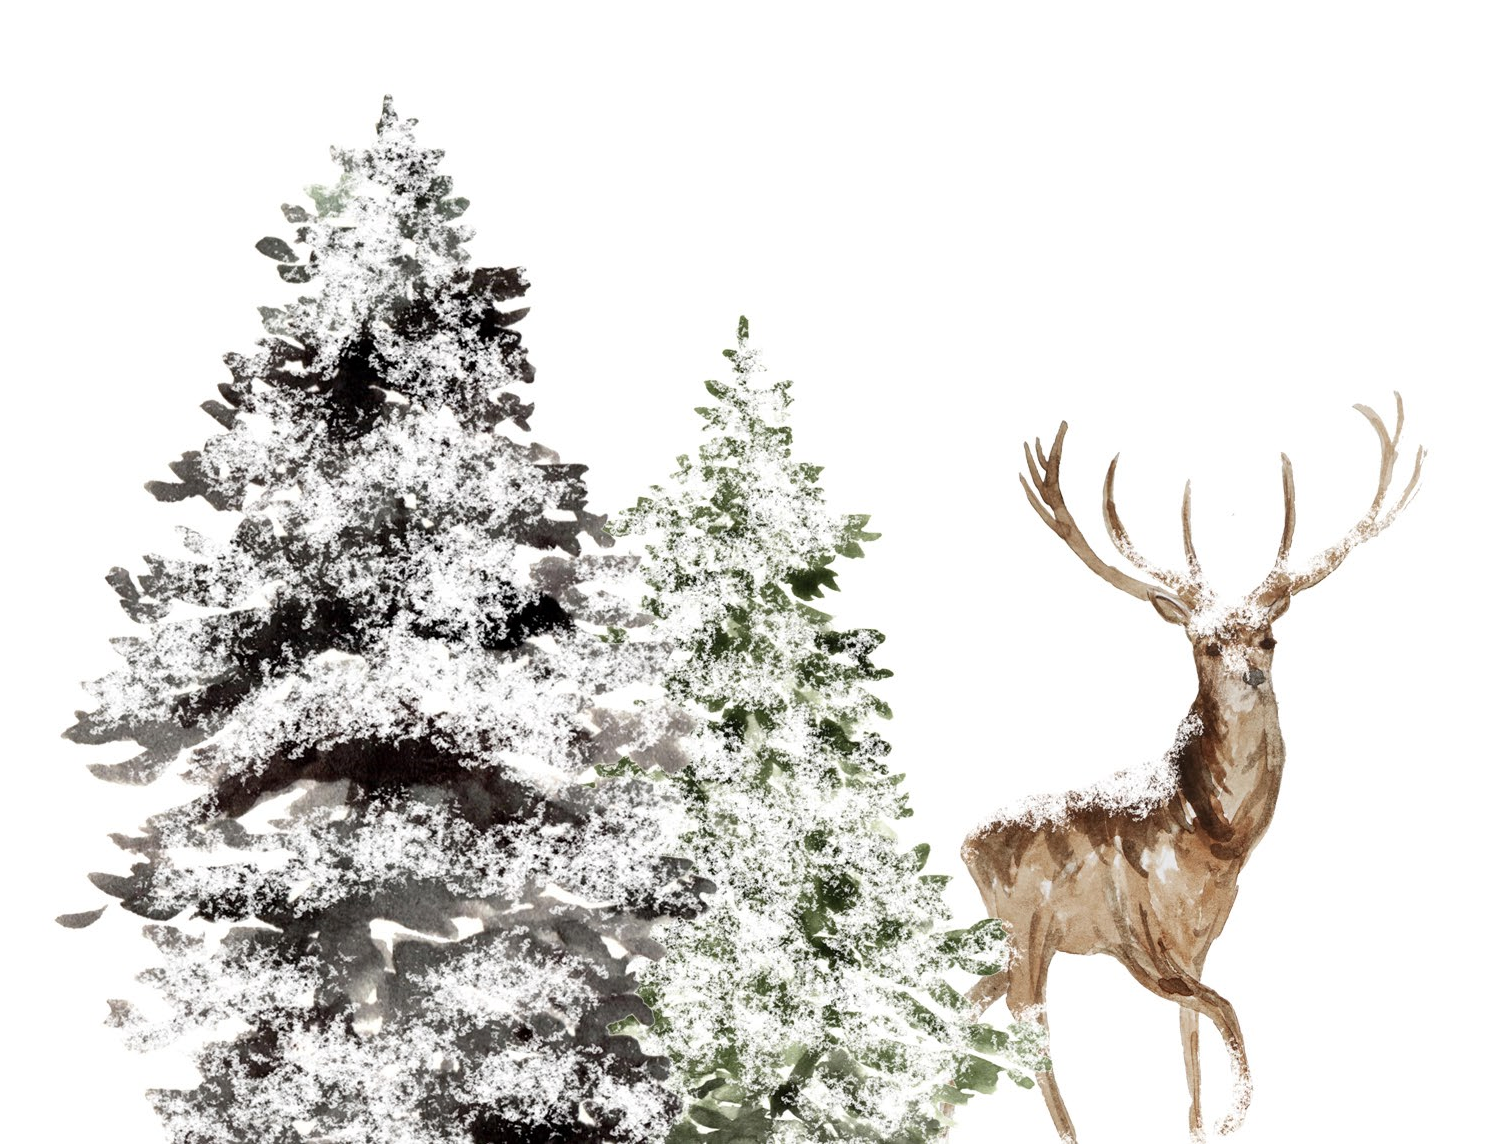
\includegraphics[width=\columnwidth]{images/deer-2}\\!
See the flowing bowl before us,\\
Fa, la, la, la, la, la, la, la, la!\\
Strike the harp and join the chorus.\\
Fa, la, la, la, la, la, la, la, la!\\
Follow me in merry measure,\\
Fa, la, la, la, la, la, la, la!\\
While I sing of beauty's treasure,\\
Fa, la, la, la, la, la, la, la, la!\\!

Fast away the old year passes,\\
Fa, la, la, la, la, la, la, la, la!\\
Hail the new, ye lads and lasses!\\
Fa, la, la, la, la, la, la, la, la!\\
Laughing, quaffing all together,\\
Fa, la, la, la, la, la, la, la!\\
Heedless of the wind and weather,\\
Fa, la, la, la, la, la, la, la, la!\\!
\end{verse}
\end{multicols}
\pagebreak
